\documentclass[a4paper,12pt]{extarticle}
\def\source{templates}
\usepackage{cmap}
\usepackage[T2A]{fontenc}
\usepackage[utf8x]{inputenc}
% Что в имени тебе моем?
% Оно умрет, как шум печальный
% Волны, плеснувшей в берег дальний,
% Как звук ночной в лесу глухом.

% Оно на памятном листке
% Оставит мертвый след, подобный
% Узору надписи надгробной
% На непонятном языке.

% Что в нем? Забытое давно
% В волненьях новых и мятежных,
% Твоей душе не даст оно
% Воспоминаний чистых, нежных.

% Но в день печали, в тишине,
% Произнеси его тоскуя;
% Скажи: есть память обо мне,
% Есть в мире сердце, где живу я.
\usepackage[mode=buildnew]{standalone}

\usepackage
	{
		amssymb,
		% misccorr,
		amsfonts,
		amsmath,
		amsthm,
		wrapfig,
		makecell,
		multirow,
		indentfirst,
		ulem,
		graphicx,
		subcaption,
		float,
		esint,
		esdiff,
		tikz,
		caption,
		tikz-3dplot,
		csvsimple,
		color,
		booktabs,
		pgfplotstable,
		pgfplots,
		fancyhdr,
	}  
\usepackage[mode=buildnew]{standalone}% requires -shell-escape


\usepackage[outline]{contour}



\linespread{1.3} 
\frenchspacing 

 
\usetikzlibrary
	{
		decorations.pathreplacing,
		decorations.pathmorphing,
		patterns,
		calc,
		scopes,
		arrows,
		fadings,
		through,
		shapes.misc,
		arrows.meta,
		3d,
		quotes,
		angles,
		babel
	}


\tikzset{
	force/.style=	{
		>=latex,
		draw=blue,
		fill=blue,
				 	}, 
	%				 	
	axis/.style=	{
		densely dashed,
		blue,
		line width=1pt,
		font=\small,
					},
	%
	th/.style=	{
		line width=1pt},
	%
	acceleration/.style={
		>=open triangle 60,
		draw=magenta,
		fill=magenta,
					},
	%
	inforce/.style=	{
		force,
		double equal sign distance=2pt,
					},
	%
	interface/.style={
		pattern = north east lines, 
		draw    = none, 
		pattern color=gray!60,
					},
	cross/.style=	{
		cross out, 
		draw=black, 
		minimum size=2*(#1-\pgflinewidth), 
		inner sep=0pt, outer sep=0pt,
					},
	%
	cargo/.style=	{
		rectangle, 
		fill=black!70, 
		inner sep=2.5mm,
					},
	%
	caption/.style= {
		midway,
		fill=white!20, 
		opacity=0.9
					},
	%
	}


\newcommand{\irodov}[2]{\geometry{left=1cm,right=1cm,top=2cm,bottom=1.5cm,bindingoffset=0cm}
\pagestyle{fancy}\fancyhead{}\fancyhead[C]{#2}\fancyhead[R]{Сарафанов Ф.Г.}  \fancyhead[L]{Иродов -- №#1}\fancyfoot{} \fancyfoot[C]{\thepage}}
\newcommand{\yakovlev}[2]{\geometry{left=1cm,right=1cm,top=2cm,bottom=1.5cm,bindingoffset=0cm}
\pagestyle{fancy}\fancyhead{}\fancyhead[C]{#2}\fancyhead[R]{Сарафанов Ф.Г.}  \fancyhead[L]{Яковлев -- №#1}\fancyfoot{} \fancyfoot[C]{\thepage}}
\newcommand{\wrote}[2]{\geometry{left=1cm,right=1cm,top=2cm,bottom=1.5cm,bindingoffset=0cm}
\pagestyle{fancy}\fancyhead{}\fancyhead[C]{#2}\fancyhead[R]{Сарафанов Ф.Г.} \fancyhead[L]{Под запись -- <<#1>>}\fancyfoot{} \fancyfoot[C]{\thepage}}

\newcommand{\siv}[2]{\geometry{left=1cm,right=1cm,top=2cm,bottom=1.5cm,bindingoffset=0cm}
\pagestyle{fancy}\fancyhead{}\fancyhead[C]{#2}\fancyhead[R]{Сарафанов Ф.Г.} \fancyhead[L]{Сивухин -- №#1}\fancyfoot{} \fancyfoot[C]{\thepage}}




\newcommand{\irodovT}[1]{\geometry{left=1cm,right=1cm,top=2cm,bottom=1.5cm,bindingoffset=0cm}
\pagestyle{fancy}\fancyhead{}\fancyhead[C]{ТД}\fancyhead[R]{Сарафанов Ф.Г.}  \fancyhead[L]{Иродов -- №#1}\fancyfoot{} \fancyfoot[C]{\thepage}}

\newcommand{\irodovE}[1]{\geometry{left=1cm,right=1cm,top=2cm,bottom=1.5cm,bindingoffset=0cm}
\pagestyle{fancy}\fancyhead{}\fancyhead[C]{Электростатика}\fancyhead[R]{Сарафанов Ф.Г.}  \fancyhead[L]{Иродов -- №#1}\fancyfoot{} \fancyfoot[C]{\thepage}}


\newcommand{\yakovlevT}[1]{\geometry{left=1cm,right=1cm,top=2cm,bottom=1.5cm,bindingoffset=0cm}
\pagestyle{fancy}\fancyhead{}\fancyhead[C]{ТД}\fancyhead[R]{Сарафанов Ф.Г.}  \fancyhead[L]{Яковлев -- №#1}\fancyfoot{} \fancyfoot[C]{\thepage}}
\newcommand{\wroteT}[1]{\geometry{left=1cm,right=1cm,top=2cm,bottom=1.5cm,bindingoffset=0cm}
\pagestyle{fancy}\fancyhead{}\fancyhead[C]{ТД}\fancyhead[R]{Сарафанов Ф.Г.} \fancyhead[L]{Под запись -- <<#1>>}\fancyfoot{} \fancyfoot[C]{\thepage}}

\newcommand{\sivT}[1]{\geometry{left=1cm,right=1cm,top=2cm,bottom=1.5cm,bindingoffset=0cm}
\pagestyle{fancy}\fancyhead{}\fancyhead[C]{ТД}\fancyhead[R]{Сарафанов Ф.Г.} \fancyhead[L]{Сивухин -- №#1}\fancyfoot{} \fancyfoot[C]{\thepage}}

\newenvironment{tikzpict}
    {
	    \begin{figure}[htbp]
		\centering
		\begin{tikzpicture}
    }
    { 
		\end{tikzpicture}
		% \caption{caption}
		% \label{fig:label}
		\end{figure}
    }

\newcommand{\vbLabel}[3]{\draw ($(#1,#2)+(0,5pt)$) -- ($(#1,#2)-(0,5pt)$) node[below]{#3}}
\newcommand{\vaLabel}[3]{\draw ($(#1,#2)+(0,5pt)$) node[above]{#3} -- ($(#1,#2)-(0,5pt)$) }

\newcommand{\hrLabel}[3]{\draw ($(#1,#2)+(5pt,0)$) -- ($(#1,#2)-(5pt,0)$) node[right, xshift=1em]{#3}}
\newcommand{\hlLabel}[3]{\draw ($(#1,#2)+(5pt,0)$) node[left, xshift=-1em]{#3} -- ($(#1,#2)-(5pt,0)$) }



\newcommand\zi{^{\,*}_i}
\newcommand\sumn{\sum_{i=1}^{N}}


\tikzset{
	coordsys/.style={scale=1.8,x={(1.1cm,-0cm)},y={(0.5cm,1cm)}, z={(0cm,0.8cm)}},
	% coordsys/.style={scale=1.5,x={(0cm,0cm)},y={(1cm,0cm)}, z={(0cm,1cm)}}, 
	% coordsys/.style={scale=1.5,x={(1cm,0cm)},y={(0cm,1cm)}, z={(0cm,0cm)}}, 
}
\usepgfplotslibrary{units}
%Русский язык в input (если расположить раньше, будет ошибка)
% \makeatletter
%     \let\old@input\input
%     \renewcommand\input[1]{%
%         \expandafter\old@input{\detokenize{#1}}%
%     }
% \makeatother

% \usepackage{import}

% Draw line annotation
% Input:
%   #1 Line offset (optional)
%   #2 Line angle
%   #3 Line length
%   #5 Line label
% Example:
%   \lineann[1]{30}{2}{$L_1$}
\newcommand{\lineann}[4][0.5]{%
    \begin{scope}[rotate=#2, blue,inner sep=2pt, ]
        \draw[dashed, blue!40] (0,0) -- +(0,#1)
            node [coordinate, near end] (a) {};
        \draw[dashed, blue!40] (#3,0) -- +(0,#1)
            node [coordinate, near end] (b) {};
        \draw[|<->|] (a) -- node[fill=white, scale=0.8] {#4} (b);
    \end{scope}
}
\newcommand{\lineannn}[4][0.5]{%
    \begin{scope}[rotate=#2, blue,inner sep=2pt, ]
        \draw[dashed, blue!40] (0,0) -- +(0,#1)
            node [coordinate, near end] (a) {};
        \draw[dashed, blue!40] (#3,0) -- +(0,#1)
            node [coordinate, near end] (b) {};
        % \draw[color=white, color=blue] (a) -- node[fill=white, scale=0.8] {#4} (b);
        \draw[->|] (a)++(-0.3,0) -- (a);
        \draw[->|] (b)++(0.3,0) coordinate (xx) -- (b);
        \draw (xx) node[fill=white, scale=0.8, right] {#4};
    \end{scope}
}

\tikzset{
  pics/carc/.style args={#1:#2:#3}{
    code={
      \draw[pic actions] (#1:#3) arc(#1:#2:#3);
    }
  },
  dash/.style={
  	dash pattern=on 5mm off 5mm
  }
}

\newcommand{\mean}[1]{\langle#1\rangle}

\pgfplotsset{
    % most recent feature set of pgfplots
    compat=newest,
}

\newcommand\ct[1]{\text{\rmfamily\upshape #1}}
\usepackage[europeanresistors,americaninductors]{circuitikz}

\newcommand*{\const}{\ct{const}}
% Style to select only points from #1 to #2 (inclusive)
\pgfplotsset{select/.style 2 args={
    x filter/.code={
        \ifnum\coordindex<#1\def\pgfmathresult{}\fi
        \ifnum\coordindex>#2\def\pgfmathresult{}\fi
    }
}}
\usepackage{array}
\usepackage{geometry}
\usepackage[english, russian]{babel}
\geometry
	{
		left=1cm,
		right=1cm,
		top=1cm,
		bottom=2cm,
		bindingoffset=0cm,
	}


% Элементы списка второго уровня с скобочкой вместо точки
\renewcommand{\labelenumii}{\theenumii)} 

\graphicspath{{img/}}

\def\labauthor{Сарафанов Ф.Г.}
\def\labauthors{Сарафанов Ф.Г.}
\def\labnumber{218}
\def\labtheme{Измерение емкости конденсатора}
\makeatletter
\newif\if@gather@prefix 
\preto\place@tag@gather{% 
  \if@gather@prefix\iftagsleft@ 
    \kern-\gdisplaywidth@ 
    \rlap{\gather@prefix}% 
    \kern\gdisplaywidth@ 
  \fi\fi 
} 
\appto\place@tag@gather{% 
  \if@gather@prefix\iftagsleft@\else 
    \kern-\displaywidth 
    \rlap{\gather@prefix}% 
    \kern\displaywidth 
  \fi\fi 
  \global\@gather@prefixfalse 
} 
\preto\place@tag{% 
  \if@gather@prefix\iftagsleft@ 
    \kern-\gdisplaywidth@ 
    \rlap{\gather@prefix}% 
    \kern\displaywidth@ 
  \fi\fi 
} 
\appto\place@tag{% 
  \if@gather@prefix\iftagsleft@\else 
    \kern-\displaywidth 
    \rlap{\gather@prefix}% 
    \kern\displaywidth 
  \fi\fi 
  \global\@gather@prefixfalse 
} 
\newcommand*{\beforetext}[1]{% 
  \ifmeasuring@\else
  \gdef\gather@prefix{#1}% 
  \global\@gather@prefixtrue 
  \fi
} 
\makeatother
%%%%%%%%%%%%%%%%%%%%%%%%%%%%%%%%%%%%%%%%%%%%%%%%%
\geometry		
	{
		left			=	2cm,
		right 			=	2cm,
		top 			=	3cm,
		bottom 			=	3cm,
		bindingoffset	=	0cm
	}
%%%%%%%%%%%%%%%%%%%%%%%%%%%%%%%%%%%%%%%%%%%%%%%%%%%%%%%%%%%%%%%%%%%%%%%%%%%%%%%
	%применим колонтитул к стилю страницы
\pagestyle{fancy} 
	%очистим "шапку" страницы
\fancyhead{} 
	%слева сверху на четных и справа на нечетных
\fancyhead[R]{\labauthors} 
	%справа сверху на четных и слева на нечетных
\fancyhead[L]{Отчёт по лабораторной работе №\labnumber} 
	%очистим "подвал" страницы
\fancyfoot{} 
	% номер страницы в нижнем колинтуле в центре
\fancyfoot[C]{\thepage} 

%%%%%%%%%%%%%%%%%%%%%%%%%%%%%%%%%%%%%%%%%%%%%%%%%%%%%%%%%%%%%%%%%%%%%%%%%%%%%%%
\usepackage{epigraph}
% \setlength{\epigraphrule}{0pt}


	    % \pgfkeys{/pgf/number format/.cd,
		% fixed,  1000 sep={\,}}
		\pgfplotstableset{
			% multicolumn names, % allows to have multicolumn names
			% col sep=tab, % the seperator in our .csv file
			% precision=2,
			% fixed zerofill, 										
			empty cells with={\textbf{--}},
			every head row/.style={
			before row={\toprule},
			after row={
				\midrule}
				},
			every last row/.style={after row=\bottomrule},
			every row/.style={after row=\midrule}, 				
			% dec sep align,
			% dec zerofill
			% fixed,fixed zerofill,
			% precision=2
		}

\begin{document}

\begin{titlepage}

\begin{center}

{\small\textsc{Нижегородский государственный университет имени Н.\,И. Лобачевского}}
\vskip 1pt \hrule \vskip 3pt
{\small\textsc{Радиофизический факультет}}

\vfill

{\Large Отчет по лабораторной работе №\labnumber\vskip 12pt\bfseries \labtheme}
	
\end{center}

\vfill
	
\begin{flushright}
	{Выполнил студент 420 группы\\ \labauthor}%\vskip 12pt Принял:\\ Менсов С.\,Н.}
\end{flushright}
	
\vfill
	
\begin{center}
	Нижний Новгород, 2017
\end{center}

\end{titlepage}

 %Титульная страница

\tableofcontents
\newpage

\section*{Введение} % (fold)
\addcontentsline{toc}{section}{Введение}
\label{sec:input}
\epigraph{\textit{Существует лишь то, что можно измерить.}}
{Цитата приписывается Максу Планку}


 Для измерения сопротивлений, емкостей и индуктивностей  часто  применяют
компенсационный метод, заключающийся в компенсации измеряемой величины некой эталонной величиной. 

В схеме типа <<мост>> элементы цепи соединяют  <<четырехугольником>>, в одну диагональ  которого  включают  источник  напряжения,  а  в  другую  --
измерительный  прибор.  При  определенном  соотношении   между   параметрами
элементов измерительный прибор показывает отсутствие напряжения в  диагонали
(баланс моста).



\begin{figure}[H]
	\centering
	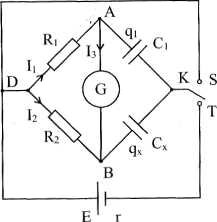
\includegraphics[width=0.5\textwidth]{img/chem}
	\caption{Принципиальная схема установки}
	\label{fig:figure1}
\end{figure}

\newpage
\section{Вывод формул}
\subsection{Напряжение на диагонали моста}

Применяя к контуру DATD второе правило Кирхгофа, получаем
\begin{equation}
i_1 R_1 + \frac{q_1}{C_1}=\varepsilon
\end{equation}
где$ i_1$ -- ток, текущий через сопротивление $R_1$, а $q_1$ -- заряд конденсатора $C_1$. 
Поскольку ток через измерительный прибор пренебрежимо мал ($R_G$ велико), то $i_1=\frac{\mathrm{d}q_1 }{\mathrm{d} t}$ и уравнение (1) принимает вид:
\begin{equation}
i_1=\frac{\mathrm{d}q_1 }{\mathrm{d} t} + \frac{q_1}{R_1 C_1}=\frac{\varepsilon}{R_1}
\end{equation}
Разделяя переменные и интегрируя:
\begin{equation}
 \int \limits^{q_1}_0 \frac{\mathrm{d} q_1}{q_1-\epsilon C_1}=-\int \limits^t_0 \frac{\mathrm{d} t}{R_1 C_1}
\end{equation}

\begin{equation}
	q(t)_1 = C_1 \varepsilon \cdot 
	% \left( 1- e ^{-\frac{t}{R_1 C_1}} \right)
	\left( 
		1-
		\exp\left[		
			-\frac{t}{R_1 C_1}
		\right]
	\right)
\end{equation}
Отсюда следует, что
\begin{equation}
	U_1(t) = \varepsilon \cdot 
	% \left( 1- e ^{-\frac{t}{R_1 C_1}}\right )
	\left( 
		1-
		\exp\left[		
			-\frac{t}{R_1 C_1}
		\right]
	\right)
\end{equation}
Аналогично рассматривая контур DBTD:
\begin{equation}
i_2 R_2 + \frac{q_2}{C_x}=\varepsilon
\end{equation}
\begin{equation}
i_2=\frac{\mathrm{d}q_2 }{\mathrm{d} t} + \frac{q_2}{R_2 C_x}=\frac{\varepsilon}{R_2}
\end{equation}
\begin{equation}
 \int \limits^{q_2}_0 \frac{\mathrm{d} q_2}{q_2-\varepsilon C_x}=-\int \limits^t_0 \frac{\mathrm{d} t}{R_2 C_x}
\end{equation}

\begin{equation}
q_x(t) = C_x \varepsilon \cdot 
\left( 
	1-
	\exp\left[		
		-\frac{t}{R_2 C_x}
	\right]
\right)
\end{equation}
\begin{equation}
U_x(t) =  \varepsilon \cdot 
\left( 
	1- 
	\exp\left[
	{-\frac{t}{R_2 C_x}}
	\right]
\right)
\end{equation}
Напряжение $U_G$ на измерительном приборе можно получить из соотношений
$\phi_1-\phi_2=U_1$; $-(\phi_2-\phi_3)=U_x$.

Получаем, что
\begin{equation}
 \phi_1-\phi_3 =U_G(t)=U_1(t)-U_x(t)= \varepsilon \cdot 
 % e ^ {-\frac{t}{R_2 C_x}} - e ^{-\frac{t}{R_1 C_1}} 
	\left( 
		\exp\left[		
			-\frac{t}{R_2 C_x}
		\right]
		-
		\exp\left[		
			-\frac{t}{R_1 C_1}
		\right]
 	\right)
\end{equation}


\subsection{Отклонение стрелки в баллистическом режиме}

Пусть мы знаем колличество витков на рамке N

Рамка помещена в постоянное магнитном поле и может поворачиваться вокруг своей оси. На неё подаётся ток $I\equiv I_G$

Сила Ампера, действующая на один виток равна $F_A=I B L$, где L -- ширина рамки

Момент, создаваемый этой силой равен $ \overrightarrow{M}=\left[ \overrightarrow{r};\overrightarrow{F_A} \right]$

Сила Ампера, действующая на всю рамку в целом тогда будет равна $F_{AO}=NIBL$

Таким образов, равнодействующий момент по модулю будет равен $M_o=HNF_A=HNIBL=IBSN$, где S -- площадь рамки

В гальванометре положение рамки фиксируется пружинами специальной формы, по которым к ней подводится измеряемый ток. На рамку действует момент сил Ампера и момент упругих сил пружинок, пропорциональный углу отклонения этой рамки от положения равновесия.
\begin{equation}
J \frac{\mathrm{d}\omega_z }{\mathrm{d} t}= I_GNSB- D \cdot \alpha
\end{equation}
$J$ -- момент инерции рамки, $\omega_z=\frac{\mathrm{d}\alpha }{\mathrm{d} t}$ -- её угловая скорость вращения.

Если ток протекает кратковременно, рамка практически не успевает отклониться. В этом случае уравнение  легко проинтегрируется:
\begin{equation}
	J \mathrm{d} \omega_z =  I_GNSB\mathrm{d} t,
\end{equation}
\begin{equation}
\omega_{z0}=\frac{NSB}{J} \cdot \int I_G dt= \frac{NSB}{J}Q ,
\end{equation} 
  где $ \omega_{z0}$ -- угловая скорость, полученная рамкой, Q -- заряд, прошедший через гальванометр. После прекращения действия сил Ампера рамка, продолжая вращаться, отклоняется на некоторый угол, который можно найти, используя закон сохранения энергии:
  \begin{equation}
  \frac{J\omega_{z0}^2}{2}= \frac{D\alpha^2_{max}}{2}
   \end{equation}
Откуда
  \begin{equation}
\alpha_{max}=\frac{NSB}{\sqrt{JD}}\cdot Q 
  \end{equation}

Принципиально важно, что отклонение пропорционально заряду, протекшему через гальванометр.

\section{Результаты эксперимента}
\subsection{Зависимость времени заряда от $R_1C_1$} % (fold)
% \label{ssub:измерение_при_безинерционном_наблюдении}



    
\begin{table}[H]
	    % \caption{Экспериментальный подбор разбро}
	    \label{tab:diod}
		\centering
		\pgfplotstabletypeset[
			columns/r1/.style={
				column name={$R_1$, кОм},
			},
			columns/t/.style={
				column name={$t/k$, мс},
			},
			columns/dt/.style={
				column name={$\Delta t$, мс},
			},
			columns/mn/.style={
				column name={Множитель $k$},
			},
			columns/nu/.style={
				column name={$\nu$, Гц},
			},		
			columns/tt/.style={
				column name={$t$, мс},
			},						
			columns={r1,t,mn,dt,nu,tt},	 	
		]{data/rnu.dat}
\end{table}

\begin{figure}[H]
	\centering
	\begin{tikzpicture}[scale=1.4]
		    \begin{axis}[
			grid=both,
			% scale=2.35,
			% xmode=log,
			grid style={line width=.1pt, draw=gray!10},
			major grid style={line width=.2pt,draw=gray!50},
			% axis lines=middle,
			minor tick num=5,
			xmin=0, 
			% xmax=11,
			ymin=1,
			% ymax=5,
			xlabel={$RC$, кОм$\cdot$мкФ},
			ylabel={$t$, мс},
			tick style={very thick},
		    % scale=0.5,
		    grid=both,
		    grid style={line width=1pt, draw=black!20},
		    major grid style={line width=.5pt,draw=black!90},
		    minor y tick num=4,
		    minor x tick num=4,   
		    xtick distance=1,
		    ytick distance=1,
		    % ymax = 1.8,
		    % xmin = 100,
		    % ymin = 0,
		    % xmax = 40,
		    ticklabel style={font=\normalsize,fill=white},    
		    axis lines=middle, 	
		    xlabel style={below right, xshift=1em, font=\normalsize},
		    ylabel style={above left, font=\normalsize},		    		
			% legend style={
			% at={(rel axis cs:0,1)},
			% anchor=north west,draw=none,inner sep=0pt,fill=gray!10}
		]
	        \addplot +[mark=*, mark size=4pt, ] table [x=r1, y=tt] {data/rnu.dat};
	        % \addlegendentry{$U_c=-7$ В}


	        % \addplot [samples=100, domain=0:52] {0.05215*e^(-(x-27)^2/2/(7.5)^2)};
	        % \addlegendentry{$\sigma_k=7.5$}

	        % \addplot [samples=100, domain=0:52, dashdotdotted] {0.05215*e^(-(x-27)^2/2/(7.649)^2)};
	        % \addlegendentry{$\sigma_k=7.649$}
		    \end{axis}
		\end{tikzpicture}	
	% \caption{Caption here}
	\label{fig:figure1}
\end{figure}



\subsubsection{Измерение при сигнале типа <<меандр>>}

\begin{table}[H]
	    % \caption{Экспериментальный подбор разбро}
	    \label{tab:diod}
		\centering
		\pgfplotstabletypeset[
			columns/r1/.style={
				column name={$R_1$, Ом},
			},
			columns/r2l/.style={
				column name={$R'_1$, Ом},
			},
			columns/r2r/.style={
				column name={$R''_1$, Ом},
			},
			columns/dr/.style={
				column name={$\Delta R_2$, Ом},
			},
			columns/rsr/.style={
				column name={$\mean{R_2}$, Ом},
			},
			columns/c2/.style={
				column name={$C_2$, мкФ},
			},			
			columns={{r1}, {r2l}, {r2r}, {dr}, {rsr}, {c2}},	 	
		]{data/nur.dat}
\end{table}


\subsubsection{Измерение при постоянном напряжении $U=15$ В}
\begin{table}[H]
	    % \caption{Экспериментальный подбор разбро}
	    \label{tab:diod}
		\centering
		\pgfplotstabletypeset[
			columns/r1/.style={
				column name={$R_1$, Ом},
			},
			columns/r2l/.style={
				column name={$R'_1$, Ом},
			},
			columns/r2r/.style={
				column name={$R''_1$, Ом},
			},
			columns/dr/.style={
				column name={$\Delta R_2$, Ом},
			},
			columns/rsr/.style={
				column name={$\mean{R_2}$, Ом},
			},
			columns/c2/.style={
				column name={$C_2$, мкФ},
			},			
			columns={{r1}, {r2l}, {r2r}, {dr}, {rsr}, {c2}},	 	
		]{data/nur15.dat}
\end{table}

\subsubsection{Измерение при постоянном напряжении $U=45$ В}
\begin{table}[H]
	    % \caption{Экспериментальный подбор разбро}
	    \label{tab:diod}
		\centering
		\pgfplotstabletypeset[
			columns/r1/.style={
				column name={$R_1$, Ом},
			},
			columns/r2l/.style={
				column name={$R'_1$, Ом},
			},
			columns/r2r/.style={
				column name={$R''_1$, Ом},
			},
			columns/dr/.style={
				column name={$\Delta R_2$, Ом},
			},
			columns/rsr/.style={
				column name={$\mean{R_2}$, Ом},
			},
			columns/c2/.style={
				column name={$C_2$, мкФ},
			},			
			columns={r1, r2l, r2r, dr, rsr, c2},	 	
		]{data/nur45.dat}
\end{table}



\end{document}
